% ============================================================================
% Section 8: Implementation
% ============================================================================

\section{Implementation}
\label{sec:implementation}

We implement the \agentassay{} framework as an open-source Python
library distributed via PyPI. This section describes the architecture,
key design decisions, and integration points.

\subsection{Architecture Overview}
\label{sec:implementation:arch}

\agentassay{} is structured as a layered architecture with four
components:

\begin{enumerate}[leftmargin=*]
  \item \textbf{Core Engine.} Implements the stochastic test semantics
    (\cref{sec:stochastic}): verdict computation, regression detection,
    SPRT, Bayesian analysis, and multiple-testing correction.

  \item \textbf{Coverage Analyzer.} Computes the five-dimensional
    coverage tuple (\cref{sec:coverage}) from execution traces. Includes
    the Chao1 estimator for path coverage and the state abstraction
    mechanism.

  \item \textbf{Mutation Engine.} Generates mutants using the four
    operator classes (\cref{sec:mutation}), executes them with
    SPRT-accelerated kills, and computes mutation scores.

  \item \textbf{Framework Adapters.} Provide integration with agent
    frameworks. Each adapter translates the framework's execution model
    into \agentassay{}'s trace format (\cref{def:trace}).
\end{enumerate}

\begin{figure}[t]
  \centering
  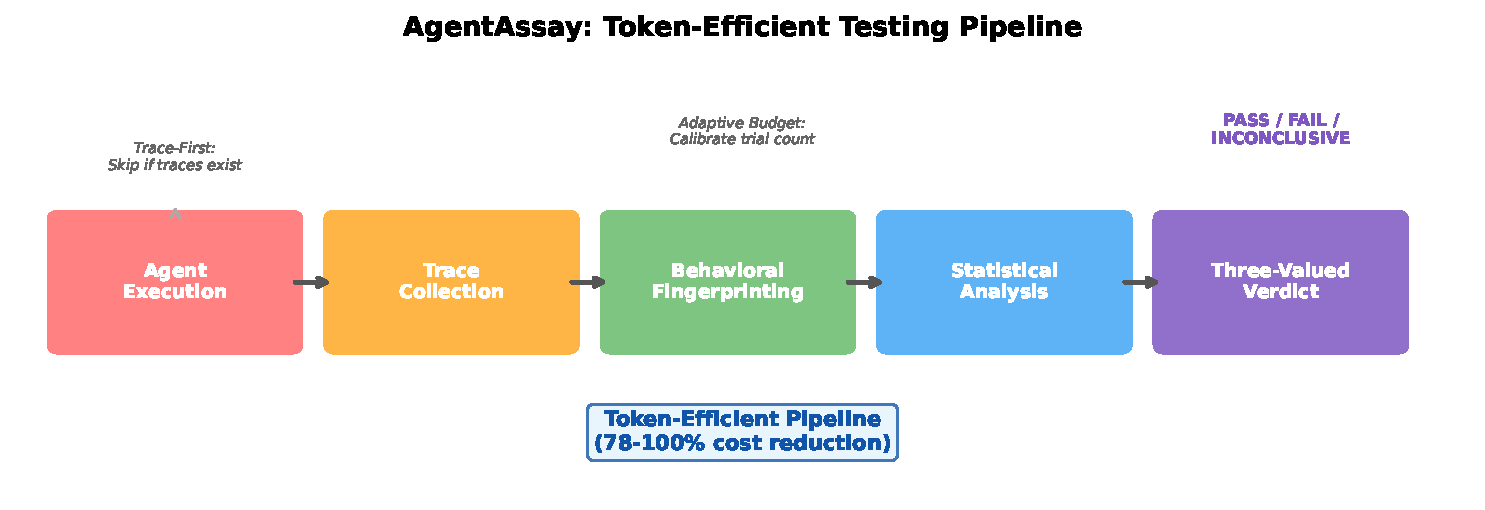
\includegraphics[width=\columnwidth]{figures/pipeline_workflow.pdf}
  \caption{\agentassay{} token-efficient testing pipeline. Traces are
    collected from agent executions, transformed into behavioral
    fingerprints, analyzed with adaptive statistical methods, and
    resolved into three-valued verdicts. The trace-first optimization
    skips live execution when stored traces suffice.}
  \label{fig:pipeline}
\end{figure}

\subsection{pytest Plugin Design}
\label{sec:implementation:pytest}

\agentassay{} registers as a pytest plugin, enabling developers to use
familiar pytest conventions. A stochastic agent test is defined using
the \texttt{@agentassay.test} decorator:

\begin{verbatim}
import agentassay

@agentassay.test(
    trials=50,
    threshold=0.85,
    alpha=0.05,
    method="sprt"
)
def test_ticket_routing(agent, scenario):
    result = agent.run(scenario.input)
    return scenario.evaluate(result)
\end{verbatim}

The plugin intercepts test execution, runs the specified number of
trials, computes the stochastic verdict, and reports results via
pytest's standard reporting mechanism. Stochastic verdicts are displayed
using custom markers:

\begin{itemize}[leftmargin=*]
  \item \PASS{}: Green checkmark with confidence interval
  \item \FAIL{}: Red cross with $p$-value and effect size
  \item \INCONC{}: Yellow warning with required additional trials
\end{itemize}

\subsection{Framework Adapters}
\label{sec:implementation:adapters}

\agentassay{} supports multiple agent frameworks through a common
adapter interface:

\begin{verbatim}
class AgentAdapter(Protocol):
    def run(self, input: str) -> AgentTrace:
        """Execute the agent and return a trace."""
        ...

    def get_tools(self) -> list[Tool]:
        """Return the agent's tool inventory."""
        ...

    def get_config(self) -> AgentConfig:
        """Return the agent's configuration."""
        ...
\end{verbatim}

We provide built-in adapters for:
\begin{enumerate}[leftmargin=*]
  \item \textbf{LangGraph}~\citep{langgraph2024}: Wraps LangGraph's
    \texttt{StateGraph} execution.
  \item \textbf{CrewAI}~\citep{crewai2024}: Wraps crew task execution
    with role-based tracing.
  \item \textbf{AutoGen}~\citep{wu2023autogen}: Wraps multi-agent
    conversation flows.
  \item \textbf{OpenAI Agents SDK}~\citep{openai2025agents}: Wraps the
    official OpenAI agent runtime.
  \item \textbf{smolagents}: Wraps Hugging Face's lightweight agent
    framework.
  \item \textbf{Semantic Kernel}: Wraps Microsoft's AI orchestration
    framework.
  \item \textbf{Amazon Bedrock Agents}: Wraps AWS Bedrock agent runtime.
  \item \textbf{MCP (Model Context Protocol)}: Wraps Anthropic's tool
    connectivity protocol.
  \item \textbf{Vertex AI Agent Builder}: Wraps Google Cloud's agent
    platform.
  \item \textbf{Generic}: A framework-agnostic adapter for any callable
    that produces structured output.
\end{enumerate}

\subsection{Test Specification Format}
\label{sec:implementation:spec}

Test scenarios are specified in YAML:

\begin{verbatim}
name: ticket_routing_accuracy
description: Route support tickets to correct department
agent: ticket_router_v2
scenarios:
  - input: "My payment failed"
    properties:
      - expected_department: billing
      - max_steps: 5
    evaluator: exact_match
  - input: "Cannot login to account"
    properties:
      - expected_department: authentication
    evaluator: exact_match

config:
  trials: 50
  threshold: 0.90
  alpha: 0.05
  beta: 0.10
  method: sprt
  regression:
    baseline: ./baselines/v1.json
    delta: 0.10
\end{verbatim}

\subsection{Contract Integration with AgentAssert}
\label{sec:implementation:contracts}

\agentassay{} integrates with the \agentassert{}
framework~\citep{bhardwaj2026abc} through the \contractspec{} DSL.
Behavioral contracts serve as formal test oracles:

\begin{verbatim}
# ContractSpec contract as evaluator
evaluator:
  type: contract
  contract: ./contracts/ticket_router.yaml
  clause: response_accuracy
\end{verbatim}

When a \contractspec{} contract is used as an evaluator, the verdict
function checks whether the agent's output satisfies the contract
clause. This connection enables the verdict-contract correspondence
(\cref{prop:verdict-contract}): a \PASS{} verdict implies contract
compliance with statistical guarantees.

\subsection{Report Generation}
\label{sec:implementation:reports}

\agentassay{} generates three types of reports:

\begin{enumerate}[leftmargin=*]
  \item \textbf{Terminal report.} Rich CLI output showing verdicts,
    confidence intervals, $p$-values, effect sizes, and coverage metrics
    for each scenario.

  \item \textbf{HTML report.} Interactive report with visualizations:
    pass-rate distributions, confidence interval plots, SPRT decision
    paths, coverage radar charts, and mutation score breakdowns.

  \item \textbf{JUnit XML.} Standard JUnit XML for CI/CD integration.
    Stochastic metadata (confidence intervals, $p$-values) is encoded in
    test properties.
\end{enumerate}

\subsection{Implementation Statistics}
\label{sec:implementation:stats}

\begin{table}[t]
\centering
\caption{Implementation statistics for \agentassay{}.}
\label{tab:impl-stats}
\small
\begin{tabular}{lr}
\toprule
\textbf{Component} & \textbf{Lines of Code} \\
\midrule
Core Engine (statistics, verdicts) & 3{,}092 \\
Coverage Analyzer & 844 \\
Mutation \& Metamorphic Engine & 3{,}710 \\
Token-Efficient Engine & 2{,}324 \\
Framework Adapters (10 frameworks) & 4{,}469 \\
Infrastructure (CLI, dashboard, persistence) & 5{,}644 \\
\midrule
\textbf{Implementation Total} & \textbf{20{,}146} \\
Test Suite (751 tests) & 7{,}384 \\
\midrule
\textbf{Grand Total} & \textbf{27{,}530} \\
\bottomrule
\end{tabular}
\end{table}
